\chapter{Muon Drift Tube Luminosity}

Overview , past experience, motivation

\section{Detector Layout}
Description of the DT system layout, trigger primitive objects

\section{Trigger Primitive Counting and Data Acquisition}
DT backend, trigger primitive counting, and  data transfer

\section{Expected Performance}
Rates, linearity, statistical precision

\clearpage
\newpage
\begin{figure}[hbtp]
\centering
\begin{subfigure}
  \centering
  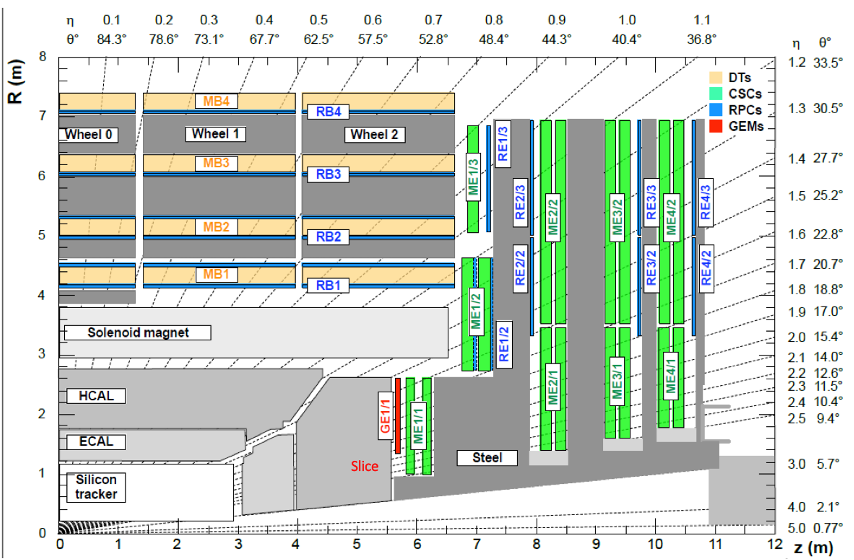
\includegraphics[width=.9\linewidth]{tex/Part2/DT-longitudinal.png}
\end{subfigure}
\begin{subfigure}
  \centering
  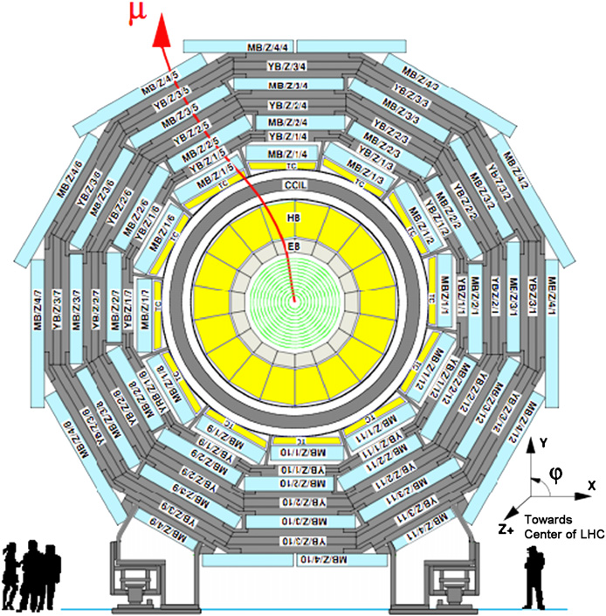
\includegraphics[width=.6\linewidth]{tex/Part2/DT-transverse.png}
\end{subfigure}
\caption{Geometrical layout of the CMS Muon barrel detector system showing the Drift Tube (DT) chambers longitudinal view (top) and transverse view (bottom). The numbering scheme for the chambers is shown in within the figure.}
\label{fig:DT_layout}
\end{figure}


\begin{figure}[hbtp]
\centering
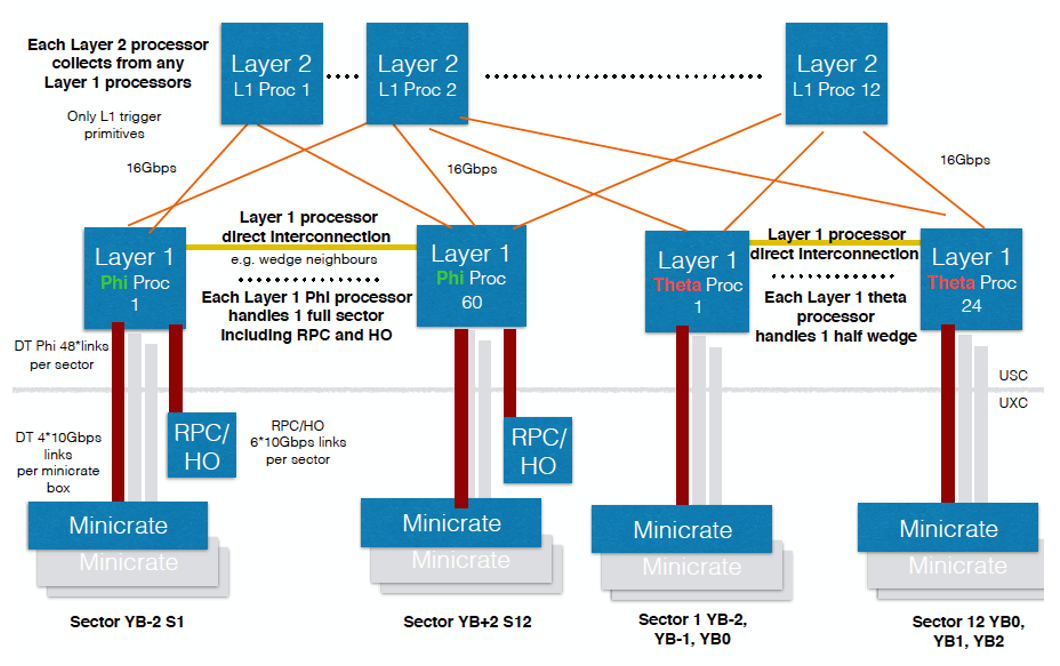
\includegraphics[width=.65\linewidth]{tex/Part2/DT-DAQoverview.png}
\caption{Design  of the Muon DAQ system architecture for Phase II showing the different layers where the L1 trigger objects are generated. In  this layout the DT trigger primitives are generated in the Layer 1 of the backend.}   
\label{fig:DT_DAQ}
\end{figure}


\begin{figure}[hbtp]
\centering
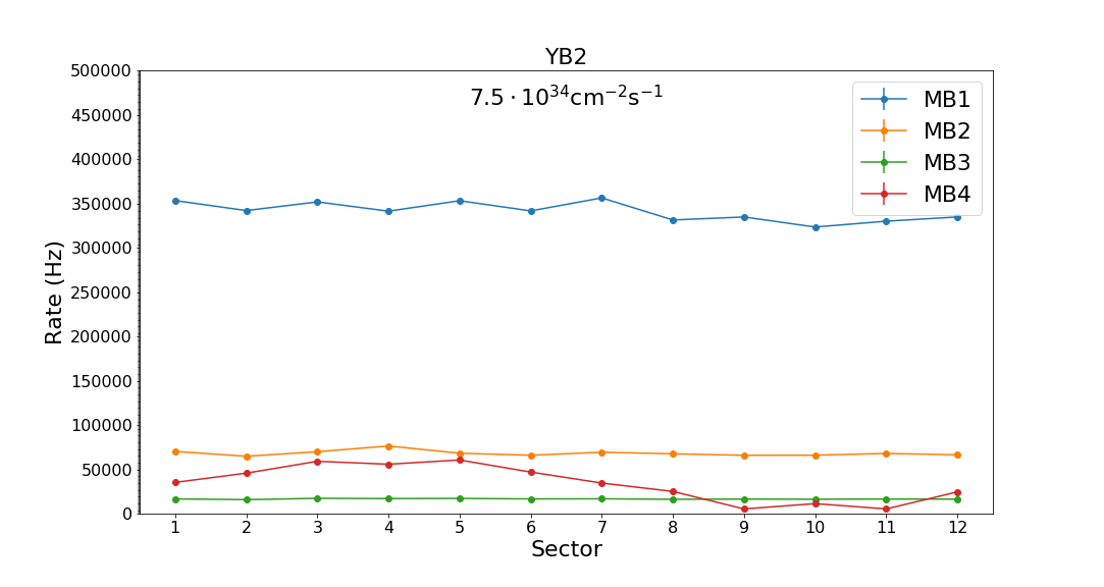
\includegraphics[width=.7\linewidth]{tex/Part2/DT-RatesExtrapolated.png}
\caption{DT L1 trigger primitive rates for the chambers in the wheel YB+2.} 
\label{fig:DT_rates}
\end{figure}


\begin{figure}[hbtp]
\centering
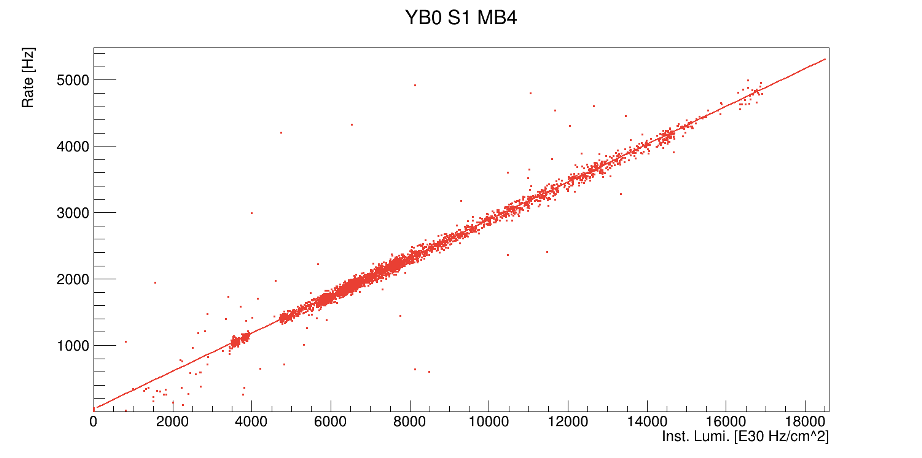
\includegraphics[width=.7\linewidth]{tex/Part2/DT-Linearity.png}
\caption{DT L1 trigger primitive rates for one chamber  as a function of instantenous luminosity measured by the HF luminometer in Run 2 data.} 
\label{fig:DT_linearity}
\end{figure}
